\documentclass[aps,prb,reprint,superscriptaddress,nofootinbib,longbibliography,floatfix]{revtex4-2}

\usepackage[utf8]{inputenc}
\usepackage[T1]{fontenc}
\usepackage{lmodern}
\usepackage{amsmath,amssymb}
\usepackage{bm}
\usepackage[final]{graphicx}
\usepackage{xcolor}
\usepackage[colorlinks=true,linkcolor=blue!55!black,citecolor=blue!55!black,urlcolor=blue!55!black]{hyperref}

\graphicspath{{figures/}}

% The same document class, fonts, colours and float settings as the report on project 1.
\renewcommand{\topfraction}{0.9}
\renewcommand{\dbltopfraction}{0.9}
\renewcommand{\bottomfraction}{0.8}
\renewcommand{\textfraction}{0.07}
\renewcommand{\floatpagefraction}{0.75}
\renewcommand{\dblfloatpagefraction}{0.75}
\setcounter{topnumber}{3}
\setcounter{dbltopnumber}{3}
\setcounter{bottomnumber}{2}
\setcounter{totalnumber}{5}

% Paragraph columns in tables are set ragged-right, with \\ still ending the row. (The array package is not
% used: with the current version, revtex 4.2f breaks paragraph columns inside ruledtabular.)
\makeatletter
\let\orig@startpbox\@startpbox
\def\@startpbox#1{\orig@startpbox{#1}\raggedright\let\\\tabularnewline}
\makeatother

\newcommand{\MSE}{\mathrm{MSE}}
\newcommand{\Mf}{\mathrm{MSE}_{g}}
\newcommand{\diag}{\mathrm{diag}}

\raggedbottom
\makeatletter
\setlength{\@fptop}{0pt}
\setlength{\@fpsep}{12pt}
\setlength{\@fpbot}{0pt plus 1fil}
\setlength{\@dblfptop}{0pt}
\setlength{\@dblfpsep}{12pt}
\setlength{\@dblfpbot}{0pt plus 1fil}
\makeatother
\begin{document}

\title{Learned or chosen features? Feed-forward neural networks for function fitting and digit recognition}

\author{Rasul Ruslanovitsj {\O}zdber}
\thanks{Parts of the text and code were produced with the assistance of a large language model; see Appendix~\protect\ref{app:llm}.}
\affiliation{Department of Physics, University of Oslo, Norway}

\date{November 9, 2026}

\begin{abstract}
Neural networks learn their features from the data, whereas polynomial and logistic regression use features fixed in advance. We study when learning the features justifies the higher cost of training, using a feed-forward network written in NumPy and verified against automatic differentiation and closed-form solutions. For 100 noisy observations of Runge's function, sigmoid networks with five or more hidden nodes had a 1.5 to 2.8 times lower mean-square deviation from the true function than the best polynomial fit, because the function's complex poles make powers of $x$ an inefficient basis. For a smooth cosine target, and for larger Runge samples with fixed network settings, polynomials were more accurate and far cheaper. On MNIST handwritten digits, one hidden layer of 512 nodes reached 98.0\% test accuracy, against 92.8\% for multinomial logistic regression. Training depended strongly on the optimizer, the activation function and the scaling of inputs and weights, whereas $L_1$ and $L_2$ penalties gave no measurable gain over early stopping. Learned features thus pay off when no good basis is known, or when the obvious one represents the target poorly.
\end{abstract}

\maketitle

\section{Introduction}\label{sec:intro}

Polynomial regression uses features chosen in advance, such as powers of the input. A neural network learns intermediate features during training. We ask when the gain in accuracy justifies the additional training cost.

With a suitable nonlinear activation, a network with one sufficiently wide hidden layer can approximate any continuous function on a compact domain \cite[Sec.~8.4]{HjorthJensen2026}. This establishes representational capacity, but does not ensure that training finds an accurate approximation.

For function fitting, we compare neural networks with ordinary least squares (OLS), Ridge, and Lasso polynomial regression. The main comparison uses the same 100 noisy observations of Runge's function as our earlier study \cite{Ozdber2026}.

On MNIST \cite{LeCun2010,LeCun1998}, we compare networks with multinomial logistic regression on the raw pixels to assess the gain from hidden layers. Across both tasks, we examine how architecture, optimization, activation, initialization, and input scaling affect training.

Our NumPy network uses backpropagation checked against automatic differentiation \cite{Harris2020}. Optimizers come from our earlier study \cite{Ozdber2026}; scikit-learn supplies preprocessing and reference estimators \cite{Pedregosa2011}.

\section{Theory}\label{sec:theory}

\subsection{Feed-forward neural networks}\label{sec:network}
A feed-forward neural network (FFNN) maps an input through successive layers. Layer 0 holds the input, layer $L$ produces the output, and layer $l$ contains $M_l$ nodes. Each node forms a weighted sum of the previous layer's outputs, adds a bias, and applies an activation function \cite[Sec.~8.5]{HjorthJensen2026},
\begin{equation}
z_j^l=\sum_{i=1}^{M_{l-1}}w_{ij}^l a_i^{l-1}+b_j^l,
\qquad a_j^l=f\!\left(z_j^l\right).
\label{eq:node}
\end{equation}
Here $a_i^0=x_i$, and $\Theta$ collects all weights and biases in a parameter vector. For $n$ samples arranged as rows, the same calculation is $\bm Z^l=\bm A^{l-1}\bm W^l+\bm b^l$, where $\bm W^l$ has shape $M_{l-1}\times M_l$ and the bias is added to each row. We describe architectures by their layer sizes: 1-50-1 has one input, one hidden layer of 50 nodes, and one output.

\subsection{Cost functions and regularization}\label{sec:costs}
Training minimizes a cost $C(\Theta)$ averaged over the samples. We write $\bm y_i$ for the target of sample $i$ and $\bm a_i^L$ for its predicted output. The regression experiments use squared error, while MNIST uses cross entropy \cite[Secs.~5.3, 5.6 and 8.7]{HjorthJensen2026}.

For regression, the output is linear, $\bm a^L=\bm z^L$, and the cost is half the mean squared error (MSE),
\begin{equation}
C_{\rm MSE}=\frac{1}{2n}\sum_{i=1}^n\left\|\bm a_i^L-\bm y_i\right\|^2,
\quad
\frac{\partial C_{\rm MSE}}{\partial\bm a_i^L}
=\frac{\bm a_i^L-\bm y_i}{n}.
\label{eq:mse}
\end{equation}
The factor $\frac12$ simplifies the gradient; the reported regression errors are the MSE itself.

For binary classification, a sigmoid output represents the probability of class 1. The binary cross entropy is the negative log-likelihood of the labels $y_i\in\{0,1\}$,
\begin{align}
C_{\rm BCE}&=-\frac1n\sum_{i=1}^n\left[y_i\ln a_i^L+(1-y_i)\ln(1-a_i^L)\right],\nonumber\\
\frac{\partial C_{\rm BCE}}{\partial a_i^L}
&=\frac{a_i^L-y_i}{n\,a_i^L(1-a_i^L)}.
\label{eq:bce}
\end{align}
For $K$ mutually exclusive classes, the softmax converts the output scores into probabilities that sum to one. With one-hot targets, $y_{ik}=1$ for the correct class and zero otherwise, the multiclass cross entropy is
\begin{align}
a_{ik}^L&=\frac{\exp(z_{ik}^L)}{\sum_{m=1}^K\exp(z_{im}^L)},\nonumber\\
C_{\rm CE}&=-\frac1n\sum_{i=1}^n\sum_{k=1}^K y_{ik}\ln a_{ik}^L,\nonumber\\
\frac{\partial C_{\rm CE}}{\partial a_{ik}^L}
&=-\frac{y_{ik}}{n\,a_{ik}^L}.
\label{eq:ce}
\end{align}

Regularization adds $\lambda\Omega(\Theta)$ to the data cost, with $\lambda\ge0$ and
\begin{equation}
\Omega_2=\sum_{\theta\in\Theta}\theta^2,
\qquad
\Omega_1=\sum_{\theta\in\Theta}|\theta|.
\label{eq:penalty}
\end{equation}
Unless stated otherwise, the sums include both weights and biases. The $L_2$ penalty adds $2\lambda\theta$ to each parameter gradient; $L_1$ adds the subgradient $\lambda\,\mathrm{sign}(\theta)$, with $\mathrm{sign}(0)=0$. The subgradient updates used here can leave small nonzero parameters under $L_1$ regularization, as examined in Appendix~\ref{app:sparsity}. Reported prediction errors exclude the penalty term. We also use early stopping, choosing the training epoch by validation performance as described in Sec.~\ref{sec:selection}.

\subsection{Activation functions}\label{sec:activation}
The hidden layers use sigmoid, rectified linear unit (ReLU), or leaky ReLU (LReLU) activations \cite[Sec.~8.6]{HjorthJensen2026},
\begin{align}
\sigma(z)&=\frac{1}{1+e^{-z}},
&\sigma'(z)&=\sigma(z)[1-\sigma(z)],\nonumber\\
\mathrm{ReLU}(z)&=\max(0,z),
&\mathrm{ReLU}'(z)&=\begin{cases}1&z>0\\0&z\le0\end{cases},\nonumber\\
\mathrm{LReLU}(z)&=\max(\alpha z,z),
&\mathrm{LReLU}'(z)&=\begin{cases}1&z>0\\\alpha&z\le0\end{cases}.
\label{eq:activations}
\end{align}
The sigmoid gives smooth responses, but saturates for large $|z|$, where its derivative approaches zero. Its derivative never exceeds $\frac14$. ReLU has unit derivative on its positive branch \cite{Nair2010}; a node with negative pre-activations for every sample receives no gradient from the data term. Leaky ReLU retains a small negative-branch slope, here $\alpha=0.01$ \cite{Maas2013}. The derivatives assigned at $z=0$ are conventions. ReLU and leaky ReLU networks are piecewise linear in their inputs, whereas sigmoid networks are smooth.

\subsection{Backpropagation}\label{sec:backprop}
Backpropagation applies the chain rule from the output layer towards the input to obtain the gradient with respect to every parameter \cite[Sec.~8.8]{HjorthJensen2026}. Consider one sample's contribution $C_s$ to the averaged data cost, so that $C=\sum_{s=1}^n C_s$, and omit the sample index on the activations. Defining $\delta_j^l=\partial C_s/\partial z_j^l$ gives
\begin{align}
\bm\delta^L&=f'\!\left(\bm z^L\right)\circ
\frac{\partial C_s}{\partial\bm a^L},\label{eq:bp1}\\
\bm\delta^l&=\left(\bm W^{l+1}\bm\delta^{l+1}\right)
\circ f'\!\left(\bm z^l\right),\label{eq:bp2}\\
\frac{\partial C_s}{\partial b_j^l}&=\delta_j^l,\label{eq:bp3}\\
\frac{\partial C_s}{\partial w_{ij}^l}&=a_i^{l-1}\delta_j^l,
\label{eq:bp4}
\end{align}
where $\circ$ denotes elementwise multiplication and the single-sample vectors are columns \cite[Sec.~8.8.4]{HjorthJensen2026}. Summing over samples gives the gradient of the data cost, to which the penalty gradient is added once. The factor $1/n$ is already included in $C_s$; for a minibatch it is replaced by the reciprocal of the actual batch size.

Equation~(\ref{eq:bp1}) assumes an elementwise output activation. For softmax, the full Jacobian is required. With each of the three output--cost pairs above, the chain rule simplifies the output error to
\[
\bm\delta^L=\frac{\bm a^L-\bm y}{n}.
\]
Appendix~\ref{app:pairs} derives these expressions. With squared error and a sigmoid or softmax output, the activation derivative or Jacobian remains in the gradient. It can make the gradient small when the output is saturated, even for a confidently wrong prediction. The MNIST experiments compare squared error with cross entropy using the same softmax output.

\subsection{Vanishing gradients and initialization}\label{sec:init}
Writing $\bm D^l=\diag[f'(\bm z^l)]$, repeated application of Eq.~(\ref{eq:bp2}) gives
\begin{equation}
\bm\delta^l=\bm D^l\bm W^{l+1}\bm D^{l+1}\cdots
\bm D^{L-1}\bm W^L\bm\delta^L.
\label{eq:product}
\end{equation}
The gradient reaching the early layers can therefore shrink or grow rapidly with depth \cite[Sec.~8.9]{HjorthJensen2026}. The rate depends on both the weight matrices and the activation derivatives. Sigmoid derivatives are at most $\frac14$ and become smaller in saturation, so repeated attenuation can leave the first layers with very small updates under plain gradient descent. ReLU avoids this attenuation on its active branch, although inactive nodes and the weight scale still affect gradient propagation.

Initial weights are Gaussian with variance $1/M_{l-1}$ for sigmoid and output layers, and $2/M_{l-1}$ for rectified layers \cite{Glorot2010,He2015}. Biases start at 0.01.

\subsection{Gradient-based optimization}\label{sec:optimizers}
The parameter updates use the optimizers from our earlier study \cite{Ozdber2026}. Gradient descent (GD) computes the gradient $\bm g_t$ over all samples and updates $\Theta_{t+1}=\Theta_t-\gamma\bm g_t$, where $\gamma$ is the learning rate. Stochastic gradient descent (SGD) applies updates using minibatches of $B$ samples \cite[Sec.~4.7]{HjorthJensen2026}. The data are reshuffled at the start of each epoch, one pass through the training set. Smaller batches give more updates per epoch, but each update uses a noisier estimate of the full gradient.

We refer to fixed-learning-rate GD and SGD as plain. RMSprop (root mean square propagation) \cite{Tieleman2012} and Adam (adaptive moment estimation) \cite{Kingma2015} instead scale each parameter's update using running gradient statistics,
\begin{align}
\text{RMSprop:}\quad
\bm s_t&=\beta\bm s_{t-1}+(1-\beta)\bm g_t^2,\nonumber\\
\Theta_{t+1}&=\Theta_t-
\frac{\gamma\bm g_t}{\sqrt{\bm s_t}+\epsilon},\nonumber\\[3pt]
\text{Adam:}\quad
\bm m_t&=\beta_1\bm m_{t-1}+(1-\beta_1)\bm g_t,\nonumber\\
\bm v_t&=\beta_2\bm v_{t-1}+(1-\beta_2)\bm g_t^2,\nonumber\\
\Theta_{t+1}&=\Theta_t-\gamma
\frac{\bm m_t/(1-\beta_1^t)}
{\sqrt{\bm v_t/(1-\beta_2^t)}+\epsilon}.
\label{eq:adaptive}
\end{align}
All operations are elementwise, and the running moments start at zero. We use $\beta=0.99$, $\beta_1=0.9$, $\beta_2=0.999$, and $\epsilon=10^{-8}$. Adam's bias corrections account for the zero initial moments. Dividing by the estimated root mean square reduces sensitivity to the gradient scale. For nearly constant gradients and negligible $\epsilon$, Adam's updates are approximately of size $\gamma$ per parameter; in general they depend on the gradient history and on $\epsilon$. This normalization can give appreciable updates in layers with small gradients. Since the network objective is generally non-convex, initialization, learning rate, and batch size can affect both convergence and the solution reached \cite[Sec.~8.15]{HjorthJensen2026}.

\subsection{Polynomial approximation of Runge's function}\label{sec:polyapprox}
Runge's function $g(x)=1/(1+25x^2)$ is smooth on $[-1,1]$, but its complex poles at $x=\pm\mathrm{i}/5$ limit the rate of polynomial approximation.

The relevant regions in the complex plane are Bernstein ellipses, with foci at $-1$ and $1$ and semiaxes $(\rho+\rho^{-1})/2$ and $(\rho-\rho^{-1})/2$, where $\rho>1$. If a function is analytic and bounded in such a region, its best degree-$d$ polynomial approximation in the maximum norm has an error bounded by a constant times $\rho^{-d}$ \cite[Chap.~8]{Trefethen2019}. For Runge's function, the limiting ellipse reaches the poles when
\[
\frac{\rho-\rho^{-1}}{2}=\frac15,
\qquad
\rho=\frac{1+\sqrt{26}}5\approx1.22.
\]
The simple poles give a geometric approximation-error scale $\rho^{-d}$. Squaring this scale gives the reference slope $\rho^{-2d}$ used in Fig.~\ref{fig:approximation}a. Since $g$ is even, the best uniform approximation can be chosen even, so increasing an even degree by one does not improve it. The squared-error scale therefore decreases by about $\rho^{-4}\approx0.45$ between successive even degrees. This is an asymptotic reference for the noise-free approximation experiment, rather than a fixed reduction guaranteed for each regression fit.

For $\cos(3x)$, polynomial approximation converges faster than any fixed geometric rate \cite[Chap.~8]{Trefethen2019}. A Chebyshev basis improves conditioning without changing the polynomial space; coefficient penalties remain basis-dependent.

\section{Methods}\label{sec:methods}

\subsection{Data}\label{sec:data}
\emph{Function fitting.}
The main regression comparison uses the same 100 noisy observations of Runge's function as our earlier study \cite{Ozdber2026},
\[
y_i=g(x_i)+\varepsilon_i,
\qquad
x_i\sim\mathcal U(-1,1),
\qquad
\varepsilon_i\sim\mathcal N(0,\sigma_\varepsilon^2),
\]
with $\sigma_\varepsilon=0.1$. The data are generated with NumPy's default generator, PCG64, and seed 2026. Two further sets of 2000 observations, generated with seeds 2027 and 2028, are used for final evaluation. The first was also used in our earlier study, and a few pilot runs inspected its errors while the experimental grids were being developed. The second was reserved for the final evaluation. We retain this distinction when interpreting the test results.

Within each training fold, we standardize the inputs and centre the targets using that fold's training statistics. The same transformations are applied to validation inputs, and predictions are shifted back by the training target mean.

\emph{Digit recognition.}
MNIST contains 60\,000 training and 10\,000 test images of handwritten digits \cite{LeCun2010}. Each $28\times28$ image is flattened to 784 pixel values and divided by 255. Our classification network uses one-hot targets. A stratified split with scikit-learn's \texttt{train\_test\_split} and seed 2026 assigns 50\,000 training images to fitting and 10\,000 to validation. Hyperparameters and training epochs are selected on this validation set. The selected models are then refitted on all 60\,000 training images before evaluation on the test set.

MNIST learning curves monitor 10\,000 fitting images and all validation images. PCG64 controls initialization and shuffling, using seed 2026 and consecutive seeds for repeats.

\subsection{Reference models}\label{sec:benchmarks}
The main Runge baselines are the polynomial models selected by cross-validation in our earlier study \cite{Ozdber2026}: degree-12 OLS, degree-12 Ridge with $\lambda_{\rm poly}=10^{-10}$, and degree-15 Lasso with $\lambda_{\rm poly}=10^{-4}$. Their inputs are polynomial features $x,\ldots,x^d$, and OLS and Ridge are fitted using closed-form solutions.

The quoted polynomial penalties retain the earlier study's convention,
$\MSE+\lambda_{\rm poly}\Omega$. The network objective uses
$\frac12\MSE+\lambda_{\rm NN}\Omega$. For otherwise identical models and penalty definitions, equivalent strengths therefore satisfy
\[
\lambda_{\rm NN}=\frac{\lambda_{\rm poly}}{2}.
\]
The distinction matters when comparing numerical penalty values across the two implementations.

For MNIST, multinomial logistic regression on the raw pixels is the main baseline. Our implementation uses the same network code with no hidden layers and a softmax output.

\subsection{Implementation}\label{sec:implementation}
The forward pass, backpropagation, and network training are implemented in NumPy \cite{Harris2020}. All weights and biases are stored in one parameter vector, allowing the optimizers and minibatch driver from our earlier study to be reused \cite{Ozdber2026}. The network class accepts the layer sizes, activation functions, cost, penalty, and initialization as arguments.

The regression estimator refits preprocessing within each fold. Autograd supplies independent gradient checks \cite{Maclaurin2015}; Matplotlib and seaborn draw saved results \cite{Hunter2007,Waskom2021}.

\subsection{Verification}\label{sec:verification}
A decreasing training loss is not sufficient evidence that backpropagation is correct. We therefore compare the gradients with independently written costs and numerical derivatives, and check limiting cases against closed-form and library solutions. Table~\ref{tab:verification} summarizes these checks. Scripts with fixed seeds save the numerical results used by the report's figures and tables.

\begin{table}[tb]
\caption{Numerical checks of the network and regression implementations.}
\label{tab:verification}
\renewcommand{\arraystretch}{1.15}
\begin{ruledtabular}
\begin{tabular}{p{0.46\columnwidth}p{0.46\columnwidth}}
Check & Result \\ \hline
Backpropagation against Autograd on an independently written cost,
for the tested activations, output--cost pairs, and penalties
& Maximum absolute gradient difference below $10^{-12}$ \\

Backpropagation against central finite differences
& Agreement within the finite-difference tolerance \\

No hidden layer and a linear output on polynomial features
& Recovers the OLS and Ridge coefficients within numerical precision \\

No hidden layer and a softmax output
& Predicted probabilities agree with scikit-learn logistic regression
within $10^{-6}$, with and without an $L_2$ penalty \\

1-50-1 sigmoid network using the seeds and settings of the course
reference implementation \cite{HjorthJensen2026week44}
& Reproduces the printed training and five-fold errors
to the last printed digit \\

Polynomial models
& Reproduce the results of our earlier study \\

One hidden layer on scikit-learn's $8\times8$ digit images
& Accuracy above 90\% and within three percentage points
of the library network \\
\end{tabular}
\end{ruledtabular}
\end{table}

\subsection{Model selection and evaluation}\label{sec:selection}
\emph{Regression.}
The main Runge models are compared using ten-fold cross-validation (CV), with identical folds for networks and polynomials \cite[Sec.~2.12]{HjorthJensen2026}. The folds are generated with shuffled \texttt{KFold} and seed 2026. Preprocessing is fitted separately within each fold.

Fold-error standard errors are $s/\sqrt{10}$. Overlapping training sets make folds dependent; these errors describe variation, not independent-sample confidence intervals or search uncertainty.

For early-stopped comparisons, we choose the recorded checkpoint with the lowest mean CV error. The selected epoch count is then used when refitting on all 100 observations.

The one-standard-error rule identifies smaller networks whose CV errors lie within one standard error of the best. For penalty searches within an architecture, it favours the largest penalty within this band \cite[Sec.~7.10]{Hastie2009}.

The Runge penalty grids use a fixed 3000 epochs. Their penalties are not combined with early stopping, so this experiment compares fixed-duration penalized fits with the early-stopped unpenalized models.

\emph{Classification.} Architecture maps use the highest validation accuracy within 15 epochs. The one-standard-error rule prefers fewer hidden nodes; penalty searches prefer the strongest penalty within the accuracy band, using each candidate's best epoch within 20 epochs.

The logistic-regression baseline is selected separately by its highest validation accuracy over the learning-rate, penalty, and epoch search. It does not use the one-standard-error rule.

Unless stated otherwise, minibatches contain 16 observations for Runge regression and 128 images for MNIST. Epoch counts measure passes through the data; they do not impose equal numbers of parameter updates or equal fit times.

\begin{figure*}[!tbp]
\centering
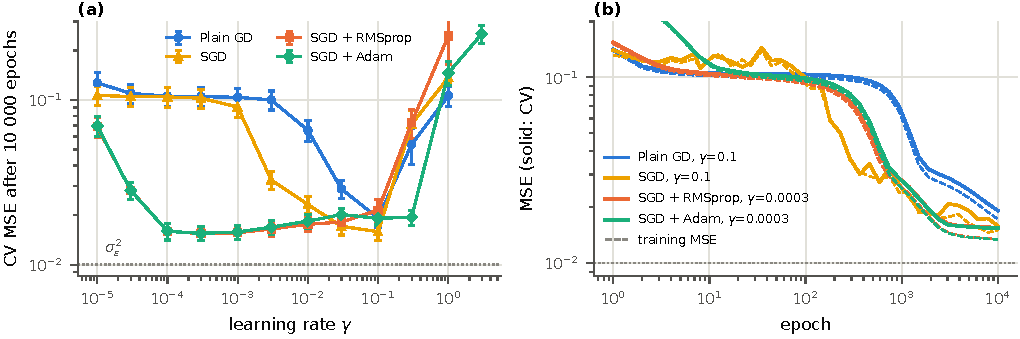
\includegraphics[width=\textwidth]{runge_learning_rate.pdf}
\caption{1-50-1 sigmoid network, 10\,000 epochs. (a) Ten-fold CV MSE with standard errors; values above 1 are omitted. (b) CV (solid) and training (dashed) errors at each optimizer's best learning rate. The dotted line marks the noise variance.}
\label{fig:lr}
\end{figure*}

\begin{figure*}[!tbp]
\centering
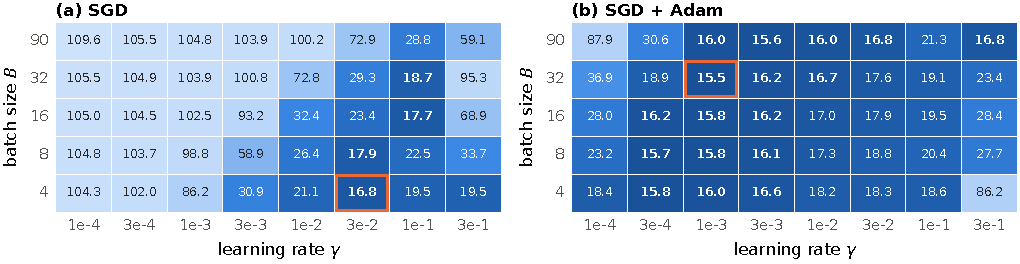
\includegraphics[width=\textwidth]{runge_batch.pdf}
\caption{CV MSE ($\times10^3$) after 3000 epochs for the 1-50-1 sigmoid network: (a) SGD, (b) Adam. Squares mark minima; bold values are within one standard error. Batch 90 is full-batch training within a fold.}
\label{fig:batch}
\end{figure*}

\emph{Prediction errors and repeated fits.}
For regression, we report MSE against the noisy test observations and, because the target function is known, the error against the underlying function,
\[
\Mf=\frac1m\sum_{i=1}^m
\left[\hat g(x_i)-g(x_i)\right]^2,
\qquad m=2000.
\]
Final regression network errors are reported as means and standard deviations over ten initializations.

For MNIST, accuracy is the fraction of correctly classified images. For a fixed trained model with observed accuracy $p$ on $n_{\rm t}$ test images, we report the binomial standard error
$\sqrt{p(1-p)/n_{\rm t}}$. Variation across five initializations is reported separately.

\subsection{Additional regression comparisons}

Without noise, degree-1--40 Chebyshev polynomials use 2001 equally spaced points; sigmoid networks use 401. Networks receive 60\,000 full-batch Adam epochs at $\gamma=3\times10^{-3}$, retaining the best of five initializations. Each model is evaluated on its fitting grid.

For each target and $n\in\{50,100,200,500,1000\}$, we generate 40 noisy data sets with paired inputs and noise, $\sigma_\varepsilon=0.1$. Ten-fold CV retunes polynomial degree 1--20 and Ridge strength $0$ or $10^k$, $k=-10,\ldots,0$.

The 50-node sigmoid network retains the main Runge learning rate and batch size. Epoch counts approximately preserve its selected update budget; another fit receives ten times as many updates. We report median target errors and interquartile ranges on 2001 grid points.

\section{Results}\label{sec:results}

\subsection{Regression of Runge's function}\label{sec:res_runge}

\subsubsection{Optimizer, learning rate and batch size}\label{sec:res_lr}

Adam and RMSprop maintained low CV errors at rates $10^{-4}$--$3\times10^{-3}$; SGD worked best at 0.03--0.1 (Fig.~\ref{fig:lr}). Their best errors were within one standard error. Full-batch GD had not reached comparable errors after 10\,000 epochs.

Batch size and learning rate interacted strongly for plain SGD (Fig.~\ref{fig:batch}a). Smaller batches gave more updates per epoch and worked best with smaller learning rates. Adam's CV error varied less over the tested combinations (Fig.~\ref{fig:batch}b).

\subsubsection{Activation function and depth}\label{sec:res_activation}
\begin{figure*}[!tbp]
\centering
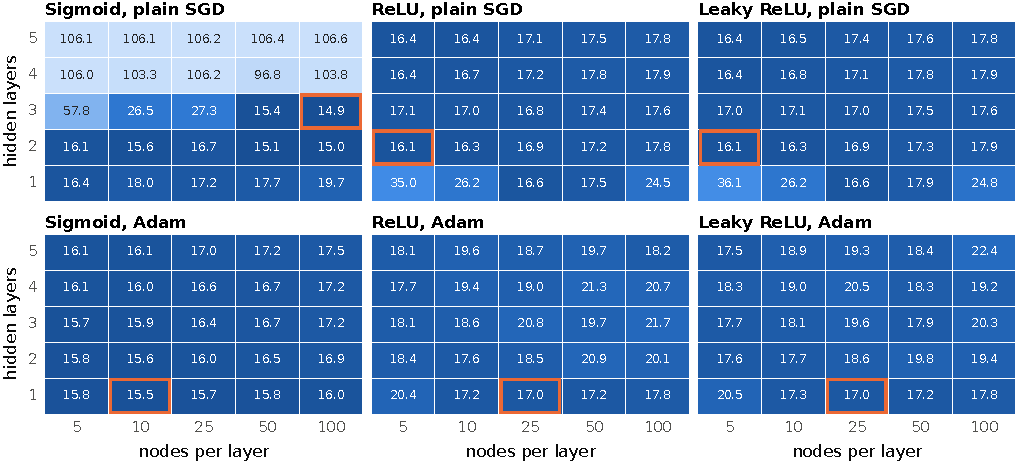
\includegraphics[width=\textwidth]{runge_activation_maps.pdf}
\caption{CV MSE ($\times10^3$) after 3000 epochs against depth and width: SGD (top), Adam (bottom). Each cell uses its best of three learning rates. Squares mark minima; the mean-prediction baseline is 106.}\label{fig:activation}
\end{figure*}
\begin{figure}[!tbp]
\centering
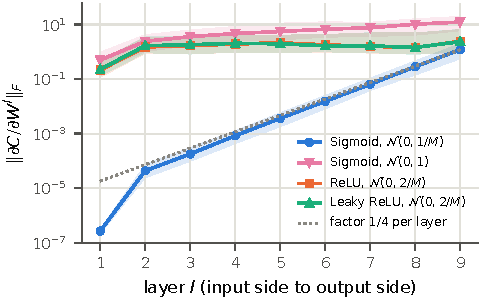
\includegraphics[width=\columnwidth]{runge_gradient_flow.pdf}
\caption{Weight-gradient Frobenius norms in untrained eight-layer, 50-node networks. Medians and interquartile ranges over 30 initializations. The dotted factor-four slope is a reference, not a universal prediction.}\label{fig:gradients}
\end{figure}

\begin{figure*}[!tbp]
\centering
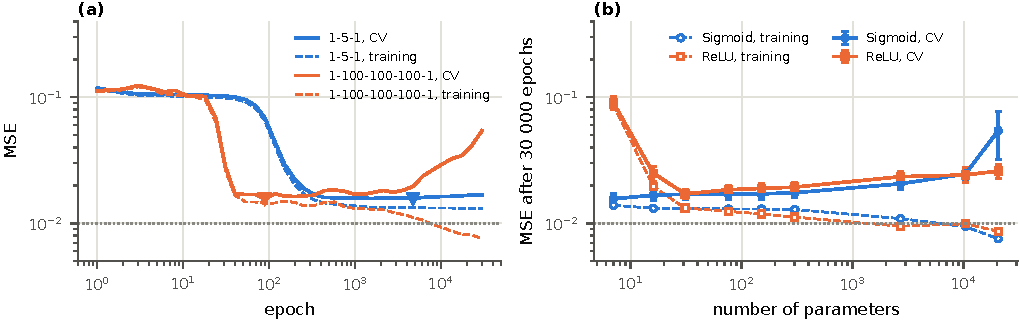
\includegraphics[width=\textwidth]{runge_overfitting.pdf}
\caption{Unpenalized Adam fits, $\gamma=3\times10^{-3}$. (a) CV (solid) and training (dashed) error; triangles mark selected checkpoints. (b) Errors after 30\,000 epochs against parameter count.}\label{fig:overfit}
\end{figure*}

\begin{figure*}[!tbp]
\centering
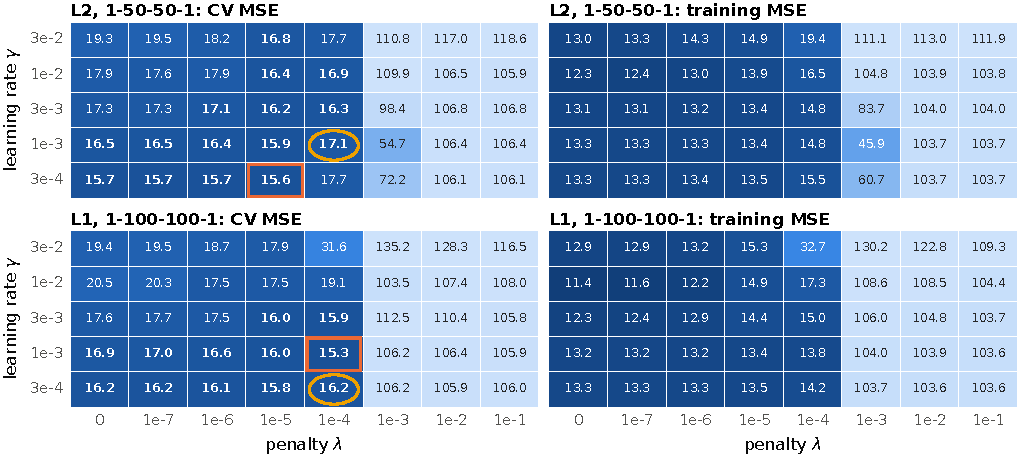
\includegraphics[width=\textwidth]{runge_penalties.pdf}
\caption{CV (left) and training (right) MSE, $\times10^3$, after 3000 epochs. Each penalty uses its best architecture. Squares mark minima; bold values are within one standard error; circles mark the one-standard-error choices.}\label{fig:penalty}
\end{figure*}

Adam gave similar CV errors across architectures, with sigmoid best; matching ReLU networks had 4--30\% higher errors (Fig.~\ref{fig:activation}). Leaky ReLU gave no systematic gain.

With plain SGD, sigmoid networks with four or five hidden layers remained near the training and CV errors of predicting the mean at every learning rate tested (Fig.~\ref{fig:activation}, top). ReLU networks trained at every tested depth.

Scaled sigmoid gradient norms decreased roughly fourfold per hidden layer, with a further 160-fold drop from the second to first layer (Fig.~\ref{fig:gradients}). This is specific to these weights and differently sized gradient matrices. ReLU showed no systematic attenuation. SGD barely changed early sigmoid layers; Adam changed all layers (Appendix~\ref{app:measurements}).

\subsubsection{Overfitting, early stopping and penalties}\label{sec:res_penalty}
\begin{table*}[!tbp]
\footnotesize
\setlength{\tabcolsep}{4pt}
\centering
\caption{Runge errors $\times10^3$. CV uses identical folds and approximate standard errors. Test errors use 2000 observations; NumPy networks show means and standard deviations over ten initializations. All networks use Adam, batch 16. Unpenalized sigmoid fits use CV-selected epochs; other NumPy networks use 3000. Times exclude search. Bold marks minima.}\label{tab:runge}
\begin{ruledtabular}
\begin{tabular}{llrcccr}
Model & Settings & Parameters & CV MSE & Test MSE & $\Mf$ & Fit time \\ \hline
OLS & degree 12 & 13 & $17.3\pm1.4$ & 11.3 & 1.62 & 0.5\,ms \\
Ridge & degree 12, $\lambda=10^{-10}$ & 13 & $17.3\pm1.4$ & 11.3 & 1.62 & 0.1\,ms \\
Lasso & degree 15, $\lambda=10^{-4}$ & 16 & $19.2\pm2.4$ & 13.2 & 3.43 & 0.13\,s \\[2pt]
1-2-1 sigmoid & $\gamma=3\times10^{-3}$, 4716 epochs & 7 & $15.6\pm1.6$ & $11.2\pm0.4$ & $1.34\pm0.46$ & 2.9\,s \\
1-5-1 sigmoid & $\gamma=3\times10^{-3}$, 4716 epochs & 16 & $15.7\pm1.4$ & $10.5\pm0.2$ & $0.60\pm0.22$ & 2.9\,s \\
1-50-1 sigmoid & $\gamma=3\times10^{-3}$, 943 epochs & 151 & $15.3\pm1.5$ & $10.7\pm0.5$ & $0.85\pm0.57$ & 1.6\,s \\
1-100-1 sigmoid & $\gamma=3\times10^{-4}$, 7897 epochs & 301 & $15.4\pm1.5$ & $\bm{10.5\pm0.2}$ & $\bm{0.58\pm0.24}$ & 6.9\,s \\
1-50-50-1 sigmoid & $\gamma=3\times10^{-3}$, 229 epochs & 2701 & $15.0\pm1.6$ & $11.1\pm0.5$ & $1.12\pm0.56$ & 0.3\,s \\
1-100-100-1 sigmoid & $\gamma=3\times10^{-4}$, 744 epochs & 10\,401 & $\bm{14.9\pm1.5}$ & $10.9\pm0.9$ & $1.06\pm1.02$ & 2.0\,s \\
1-50-50-1, $L_2$ & $\gamma=10^{-3}$, $\lambda=10^{-4}$ & 2701 & $17.1\pm2.1$ & $11.5\pm0.3$ & $1.71\pm0.35$ & 4.9\,s \\
1-100-100-1, $L_1$ & $\gamma=3\times10^{-4}$, $\lambda=10^{-4}$ & 10\,401 & $16.2\pm2.0$ & $11.1\pm0.4$ & $1.31\pm0.39$ & 10.2\,s \\
1-25-1 ReLU & $\gamma=10^{-3}$, 3000 epochs & 76 & $17.0\pm1.5$ & $11.1\pm0.4$ & $1.18\pm0.42$ & 1.5\,s \\
1-25-1 leaky ReLU & $\gamma=10^{-3}$, 3000 epochs & 76 & $17.0\pm1.5$ & $11.1\pm0.4$ & $1.18\pm0.42$ & 1.7\,s \\
Library sigmoid & $\gamma=3\times10^{-3}$, 229 epochs & 2701 & --- & 13.7 & 4.01 & 0.34\,s \\
\end{tabular}
\end{ruledtabular}
\end{table*}

\begin{figure*}[!tbp]
\centering
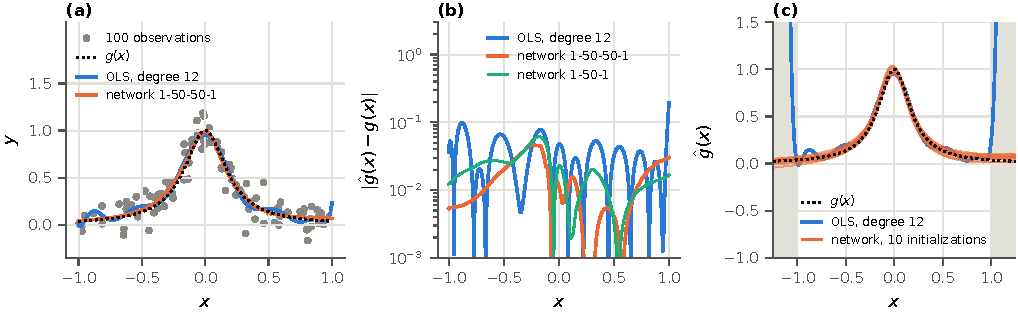
\includegraphics[width=\textwidth]{runge_fits.pdf}
\caption{Degree-12 OLS and sigmoid fits. (a) Fits, with network medians over ten initializations. (b) Error against the target. (c) Extrapolation; shading marks regions without data, thin lines individual initializations.}\label{fig:fits}
\end{figure*}

Large networks overfit during long training, but CV-selected checkpoints reduced architecture differences: sigmoid networks with 7 to over 20\,000 parameters were within one standard error of the best (Fig.~\ref{fig:overfit}).

The penalty scans gave no clear improvement over the unpenalized fits (Fig.~\ref{fig:penalty}). At $\lambda=10^{-3}$, the best CV MSE was $54.7\times10^{-3}$ with $L_2$, a substantial degradation, and $103.5\times10^{-3}$ with $L_1$, close to the mean-prediction baseline of $106\times10^{-3}$. The one-standard-error rule selected $\lambda=10^{-4}$ for both penalty types. This comparison is specific to the tested protocols: the penalized Runge models used a fixed 3000 epochs, and penalties combined with early stopping were not tested.

\subsubsection{Comparison with polynomial regression}\label{sec:res_compare}
\begin{figure*}[!tbp]
\centering
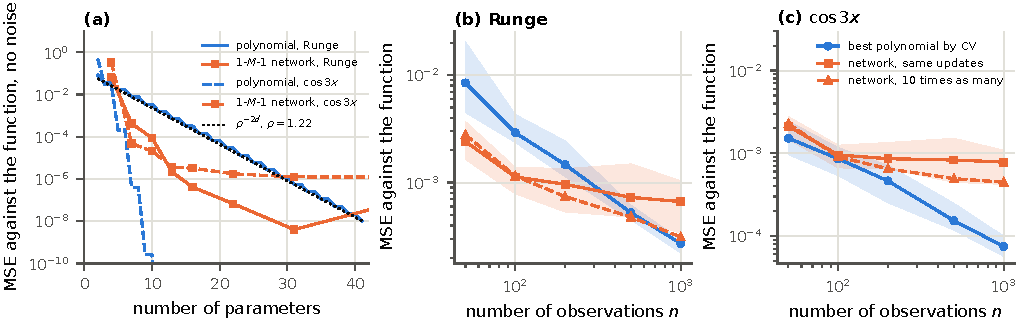
\includegraphics[width=\textwidth]{runge_approximation.pdf}
\caption{(a) Noise-free approximation errors; dotted slope $\rho^{-2d}$. (b,c) Errors over 40 noisy data sets per size, with retuned polynomials and fixed network settings at two update budgets. Lines are medians; bands are interquartile ranges, omitted for the longer budget. Protocols are in Methods.}\label{fig:approximation}
\end{figure*}

\begin{figure*}[!tbp]
\centering
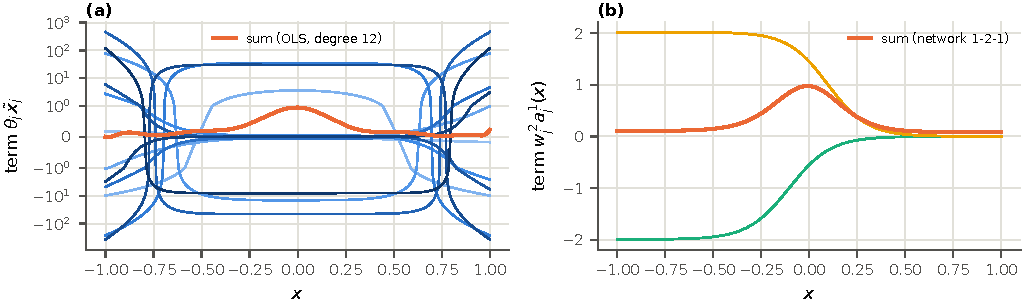
\includegraphics[width=\textwidth]{runge_features.pdf}
\caption{(a) Standardized degree-12 OLS terms on a symmetric logarithmic axis. (b) Weighted sigmoid responses of a two-node network. Constants are included in sums but not plotted separately.}\label{fig:features}
\end{figure*}

Network CV gains over OLS were small relative to standard errors (Table~\ref{tab:runge}). Paired fold differences also remain descriptive because training sets overlap and CV selected the models.

Sigmoid networks with at least five nodes had mean target errors 36--69\% of OLS; two nodes matched OLS with seven rather than thirteen parameters. All selected NumPy networks also beat OLS on the second test set. The library sigmoid reference performed worse than OLS, showing that related training settings need not reproduce the gain.

OLS errors oscillated and grew outside the data; sigmoid extrapolations stayed bounded without necessarily following the target (Fig.~\ref{fig:fits}). Network fits took 0.3--6.9\,s, versus under a millisecond for OLS and Ridge, excluding search costs.

\subsubsection{Approximation error and amount of data}\label{sec:res_approx}

Noise-free polynomial errors followed the geometric reference slope. Two sigmoid nodes achieved over ten times lower error than an equally sized polynomial. For $\cos(3x)$, ten polynomial coefficients reached about $10^{-10}$, below the tested networks (Fig.~\ref{fig:approximation}a). These comparisons depend on the stated grids and optimization protocol.

Two oppositely weighted sigmoid steps formed the Runge peak, while large monomial terms nearly cancelled (Fig.~\ref{fig:features}). The polynomial approximation limit is independent of basis.

At $n=100$, networks beat retuned polynomials on all 40 Runge repeats. At $n=1000$, polynomials won 32 repeats, falling to 22 with the longer network budget. For cosine, polynomials had lower median error at every size. At $n=500,1000$, they won all baseline-budget repeats and 36 and 39 longer-budget repeats.

\subsection{Classification of handwritten digits}\label{sec:res_mnist}

\subsubsection{Optimizer and learning rate}\label{sec:res_mnist_opt}
\begin{figure*}[!tbp]
\centering
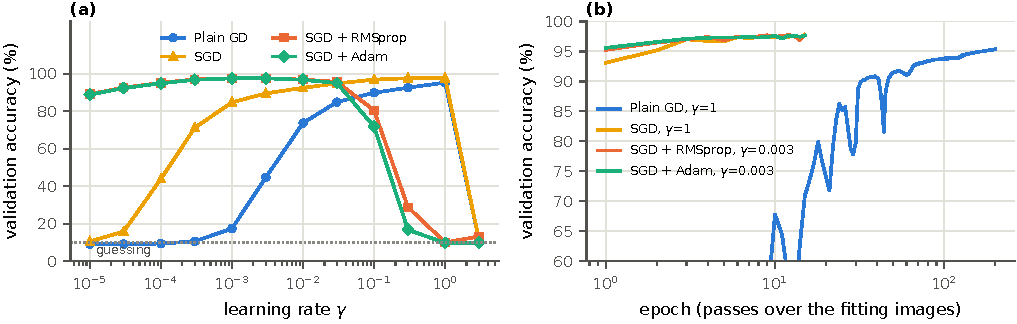
\includegraphics[width=\textwidth]{mnist_optimizers.pdf}
\caption{128-node ReLU network. (a) Validation accuracy after 15 epochs, or 200 for full-batch GD. (b) Learning curves at each optimizer's best rate. Minibatches contain 128 images.}\label{fig:mnist_opt}
\end{figure*}
\begin{figure*}[!tbp]
\centering
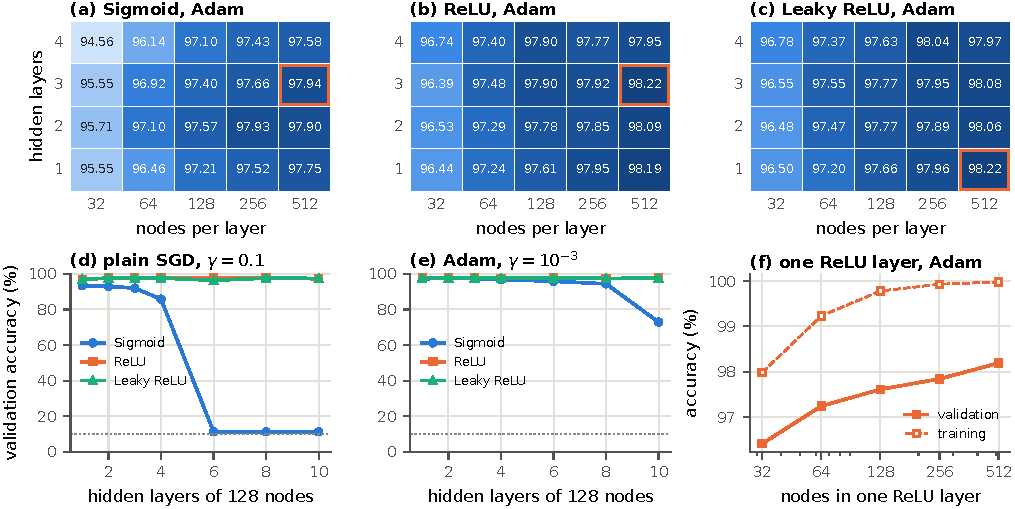
\includegraphics[width=\textwidth]{mnist_architectures.pdf}
\caption{(a--c) Best validation accuracy within 15 Adam epochs, $\gamma=10^{-3}$, against depth and width. Squares mark maxima. (d,e) Epoch-15 accuracy against depth, 128 nodes per layer. (f) Epoch-15 training-monitor and validation accuracy against ReLU width.}\label{fig:mnist_arch}
\end{figure*}

GD reached 95.37\% validation accuracy after 200 epochs. Adam exceeded this after one epoch, RMSprop after two, and SGD after three (Fig.~\ref{fig:mnist_opt}). Minibatch methods make many updates per pass; their best final accuracies were similar.

\subsubsection{Width, depth and activation}\label{sec:res_mnist_arch}
\begin{figure*}[!tbp]
\centering
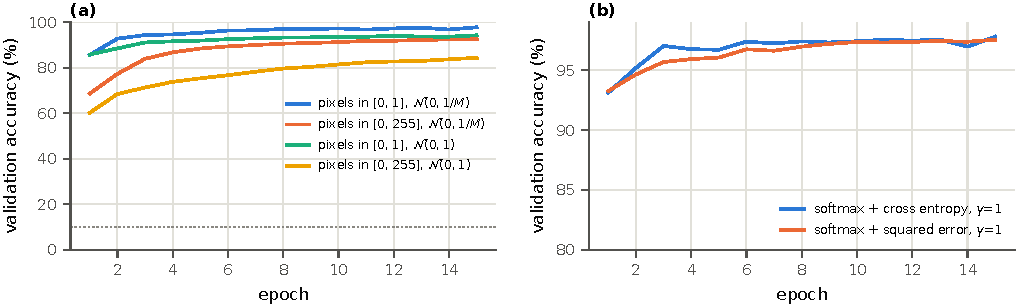
\includegraphics[width=\textwidth]{mnist_scaling_pairs.pdf}
\caption{SGD learning curves at each configuration's best tested rate. (a) Two 128-node sigmoid layers: pixels in $[0,1]$ or $[0,255]$, weight variance $1/M_{l-1}$ or 1. (b) One 128-node ReLU layer, softmax output: cross entropy versus squared error.}\label{fig:mnist_scaling}
\end{figure*}

Increasing width from 32 to 512 nodes gained about two accuracy points; depth mattered less (Fig.~\ref{fig:mnist_arch}). The one-standard-error rule selected one 512-node leaky ReLU layer. ReLU at that width also qualified; the grid did not establish an optimal width beyond 512.

With SGD, sigmoid networks of six or more hidden layers approached chance accuracy. Adam delayed this deterioration. ReLU trained at every tested depth up to ten layers.

\subsubsection{Input scaling, initialization and output cost}\label{sec:res_mnist_scaling}
\begin{figure*}[!tbp]
\centering
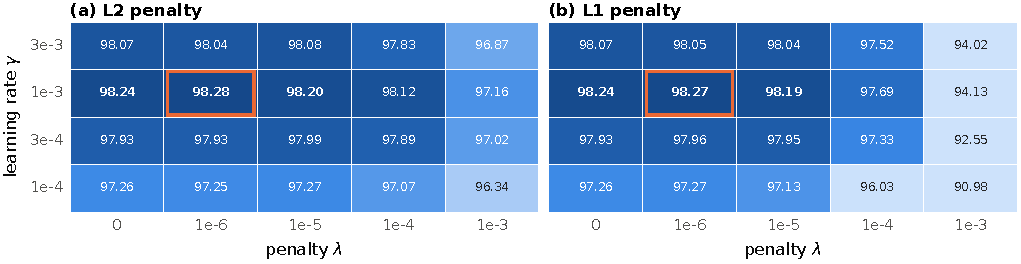
\includegraphics[width=\textwidth]{mnist_penalties.pdf}
\caption{Best MNIST validation accuracy within 20 Adam epochs, 784-512-10 leaky ReLU. Squares mark maxima; bold values lie within one binomial standard error.}\label{fig:mnist_penalty}
\end{figure*}

Raw pixels saturated 96\% of first-layer sigmoid activations initially and 98\% after training, using thresholds 0.01 and 0.99. None saturated initially with default scaling. Raw pixels cost about five accuracy points; unit-variance weights cost about 3.5 (Fig.~\ref{fig:mnist_scaling}a).

Softmax with squared error mainly slowed training (Fig.~\ref{fig:mnist_scaling}b). At uniform ten-class probabilities its gradient is ten times smaller than with cross entropy. Larger learning rates approached cross-entropy accuracy; initialization showed no confidently wrong predictions.

\subsubsection{Penalties}\label{sec:res_mnist_penalty}
\begin{figure*}[!tbp]
\centering
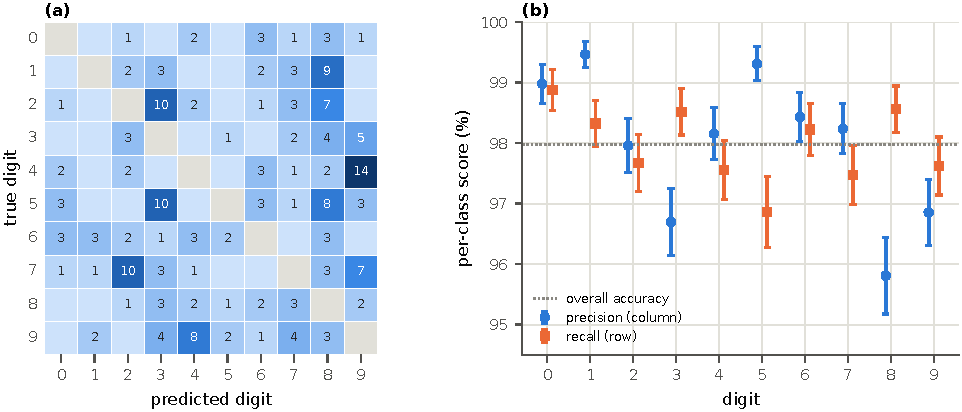
\includegraphics[width=\textwidth]{mnist_confusion.pdf}
\caption{Selected network on the test images. (a) Confusion counts, rows true and columns predicted; diagonal omitted, empty cells zero. (b) Per-digit precision and recall with binomial standard errors.}\label{fig:confusion}
\end{figure*}

\begin{figure*}[!tbp]
\centering
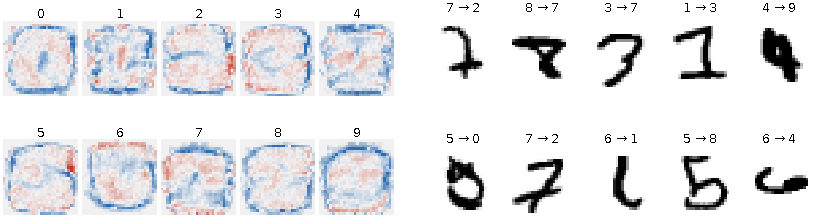
\includegraphics[width=\textwidth]{mnist_errors.pdf}
\caption{Left: logistic-regression weights as pixel templates, blue negative and red positive. Right: the network's ten most confident test errors, labelled true $\to$ predicted.}\label{fig:errors}
\end{figure*}

MNIST penalties gave no clear gain with epoch selection (Fig.~\ref{fig:mnist_penalty}). At $10^{-3}$, $L_2$ lost about one accuracy point and $L_1$ four. The one-standard-error rule selected $L_2=10^{-5}$, $\gamma=10^{-3}$, epoch 14; this does not establish an improvement over no penalty.

\subsubsection{Test accuracy and remaining errors}\label{sec:res_mnist_test}
\begin{table}[tb]
\caption{MNIST test accuracy with binomial standard errors; seed 2026, 60\,000 training images. Our selected models use Adam, $\gamma=10^{-3}$, batch 128; logistic regression uses $\lambda_2=10^{-7}$ and 25 epochs, the 512-node network $10^{-5}$ and 14 epochs. The fixed 100-node reference uses SGD, $\gamma=0.1$, batch 100, 20 epochs. Library sigmoid units differ from our leaky ReLU. Times exclude search; published training conditions differ. Bold marks the best fitted-model accuracy.}\label{tab:mnist}
\begin{ruledtabular}
\begin{tabular}{lrcr}
Model & Parameters & Accuracy & Time \\ \hline
Guessing & 0 & 10 & \\[3pt]
\multicolumn{4}{l}{\emph{Our code}} \\
Logistic regression & 7850 & $92.77\pm0.26$ & 8\,s \\
784-100-10 ReLU, SGD & 79\,510 & $97.67\pm0.15$ & 13\,s \\
784-512-10 leaky ReLU & 407\,050 & $\bm{97.98\pm0.14}$ & 6\,min \\[3pt]
\multicolumn{4}{l}{\emph{scikit-learn}} \\
Logistic regression & 7850 & $92.57\pm0.26$ & 12\,min \\
784-512-10 sigmoid & 407\,050 & $97.96\pm0.14$ & 10\,min \\[3pt]
\multicolumn{4}{l}{\emph{Published}} \\
Linear classifier & & 88.0 & \\
784-800-10 & & 98.4 & \\
LeNet-5, convolutional & & 99.05 & \\
\end{tabular}
\end{ruledtabular}
\end{table}

The selected network made 202 test errors against logistic regression's 723, a 72\% reduction (Table~\ref{tab:mnist}). Across five initializations, its accuracy was $98.06\pm0.10\%$ (standard deviation). Tables and error plots use the prespecified seed-2026 fit; binomial errors describe test-sample uncertainty.

The library sigmoid model differs in activation, initialization and bias penalties. A separate ReLU validation comparison gave $97.98\pm0.22\%$ for our code and $97.95\pm0.13\%$ for scikit-learn over five initializations (standard deviations). These compare performance; Table~\ref{tab:verification} checks correctness.

The leading confusions were four as nine (14 errors), then two and five as three and seven as two (ten each). Mean-image similarity explained only some confusions (Appendix~\ref{app:measurements}). Four-as-nine errors fell from 31 with logistic regression to 14. Precision was lowest for 8 and 3; recall for 5.

Incorrect predictions had a median assigned probability of 0.78, compared with more than 0.9999 for correct predictions. These confidence summaries describe the predictions but do not establish probability calibration.

\section{Discussion}\label{sec:discussion}

\subsection{Learned versus chosen features}\label{sec:disc_features}

Only polynomials were retuned for each new data set. The sample-size comparison therefore measures transfer of fixed network settings, not equally optimized model families.

Dense networks lack spatial weight sharing. Published convolutional results \cite{LeCun1998} suggest an alternative, but different training conditions prevent attributing their advantage solely to architecture.

\subsection{Evaluation of the methods}\label{sec:evaluation}

The fixed 100-node ReLU network reached 97.67\%, versus 97.98\% for the selected 512-node model. Different training settings and uncontrolled timings prevent interpreting this as a width-only comparison.

\begin{table*}[!tbp]
\small
\centering
\caption{Practical strengths and limitations under the tested protocols.}\label{tab:evaluation}
\renewcommand{\arraystretch}{1.15}
\begin{ruledtabular}
\begin{tabular}{@{}p{0.20\textwidth}p{0.36\textwidth}p{0.36\textwidth}@{}}
Method & Strengths & Limitations \\ \hline
Polynomial regression (OLS, Ridge, Lasso) & OLS and Ridge have fast closed-form solutions; polynomial features were effective for the cosine target & Required degree depends on the target; high-degree monomial fits can be poorly conditioned; extrapolation can be unstable \\
FFNN for regression & Sigmoid features represented the Runge peak compactly; selected models improved error against the known function & More expensive fitting and model selection; sensitivity to training settings and initialization; bounded sigmoid extrapolation need not be accurate \\
Logistic regression & Inexpensive baseline in our implementation; convex objective; class scores can be inspected as pixel templates & Class scores are linear in the supplied pixels \\
FFNN for classification & Nonlinear pixel combinations substantially reduced errors relative to the raw-pixel baseline & More parameters and training choices; dense layers have no built-in spatial weight sharing \\
Plain GD & Simple updates using the full-data gradient & One update per data pass; slow progress under the tested epoch budgets \\
Plain SGD & Many updates per pass; competitive predictive performance when tuned & Narrower useful learning-rate range; poor training of deep sigmoid networks under the tested settings \\
RMSprop and Adam & Wider useful learning-rate ranges; Adam improved training at greater sigmoid depths & Additional settings; no resolved gain in the best predictive performance from the optimizer scans alone \\
\end{tabular}
\end{ruledtabular}
\end{table*}

\section{Conclusions and outlook}\label{sec:conclusion}
Learned sigmoid features represented Runge's peak efficiently, while polynomials suited cosine and often larger samples under the tested protocol. Hidden layers substantially improved MNIST accuracy. Adaptive optimizers widened useful learning-rate ranges; penalties gave no resolved gain over the tested stopping protocols.

Future comparisons should retune both model families under equal search budgets and test convolutional MNIST networks with the same data protocol, recording selection and fitting costs.

\clearpage
\appendix

\begin{table*}[tb]
\caption{The measurements behind the explanations in the text. The relative change of a layer is $\|\bm W-\bm W_0\|/\|\bm W_0\|$ in the Frobenius norm, with $\bm W_0$ its initial weights, $\|\bm\theta-\bm\theta_0\|$ is the Euclidean norm over all parameters, and a sigmoid output counts as saturated when it is below 0.01 or above 0.99, where its derivative is below 0.01.}\label{tab:measurements}
\renewcommand{\arraystretch}{1.15}
\begin{ruledtabular}
\begin{tabular}{p{0.24\textwidth}p{0.33\textwidth}p{0.37\textwidth}}
Explanation & Measurement & Result \\ \hline
Plain SGD hardly changes the first layers of a deep sigmoid network (Sec.~\ref{sec:res_activation}) & Relative change of each layer of a network with five hidden layers of 50 sigmoid nodes after 3000 epochs on all 100 observations; median of ten initializations, at each learning rate of Fig.~\ref{fig:activation} & Plain SGD: at most 0.4\% in the first layer and 11--57\% in the output layer; the training MSE stays at that of predicting the mean. Adam: every layer changes by 0.2 to 15 times its initial size \\
Adam moves every layer of a deep sigmoid network (Sec.~\ref{sec:res_activation}) & Relative change of each layer after 15 epochs on MNIST, ten hidden layers of 128 sigmoid nodes, settings of Fig.~\ref{fig:mnist_arch}d,e & Plain SGD: 14\% in the last hidden layer, falling by a factor of about four per layer to below 0.003\% in the first four layers. Adam: every layer changes by 1.3 to 3.8 times its initial size \\
Unscaled pixels and weights saturate the sigmoid (Sec.~\ref{sec:res_mnist_scaling}) & Share of saturated outputs on the validation images, for the networks of Fig.~\ref{fig:mnist_scaling}a at their best learning rates & Scaled pixels and weights: none before training. Raw pixels: 96\% of the first layer before and 98\% after training. Weights from $\mathcal N(0,1)$: 63\% and 57\% of the two layers. Both: nearly all of the first layer \\
No prediction is confidently wrong at the start (Sec.~\ref{sec:res_mnist_scaling}) & Largest output probability of the untrained 784-128-10 network on the validation images & Median 0.16 and maximum 0.35, so no prediction is confidently wrong \\
Similar average shapes are consistent with some confusions (Sec.~\ref{sec:res_mnist_test}) & Cosine similarity of the mean training images of each pair of digits, ranked among the 45 pairs & 4 and 9 first, 3 and 5 third, 2 and 3 twelfth, 7 and 2 35th \\
Our network reaches an accuracy similar to scikit-learn's (Sec.~\ref{sec:res_mnist_test}) & Validation accuracy of our selected network and of scikit-learn's with ReLU nodes, both trained on the 50\,000 fitting images with the selected settings; five initializations each & $97.98\pm0.22\%$ and $97.95\pm0.13\%$ (mean and standard deviation) \\
In these runs, the distance moved tracks overfitting better than the number of parameters (Sec.~\ref{sec:res_penalty}) & $\|\bm\theta-\bm\theta_0\|$ along the curves of Fig.~\ref{fig:overfit}, mean over the folds & At the best epoch 7--10 for eight of the nine networks (7 to 20\,501 parameters) and 19 for 1-100-1, whose CV error hardly changes after epoch 300; after 30\,000 epochs from 7 to 200, growing with the overfitting \\
Large weights make a penalty costly (Sec.~\ref{sec:res_penalty}) & $\lambda\|\bm\theta\|^2$ of the two-node network of Fig.~\ref{fig:features}, against the data term of its cost, half its training MSE & Input weights about 5, output weights about 2; at $\lambda=10^{-3}$ the penalty, 0.06, is eight times the data term, 0.007 \\
\end{tabular}
\end{ruledtabular}
\end{table*}

\section{Matched output activations and costs}\label{app:pairs}
Equation~(\ref{eq:bp1}) multiplies the derivative of the cost by the derivative of the output activation. With a linear output $f'=1$, so Eq.~(\ref{eq:mse}) gives $\bm{\delta}^L=(\bm{a}^L-\bm{y})/n$ directly. With a sigmoid output, $\sigma'(z^L)=a^L(1-a^L)$ cancels the denominator in Eq.~(\ref{eq:bce}), and again $\delta^L=(a^L-y)/n$.

The softmax is not elementwise, because each output depends on all the scores: $\partial a_k^L/\partial z_j^L=a_k^L\left(\delta_{kj}-a_j^L\right)$, where $\delta_{kj}$ is the Kronecker delta. The chain rule with Eq.~(\ref{eq:ce}) then gives
\begin{align}
\delta_j^L&=\sum_k\frac{\partial C_{\rm CE}}{\partial a_k^L}\frac{\partial a_k^L}{\partial z_j^L}
=-\frac1n\sum_k\frac{y_k}{a_k^L}\,a_k^L\left(\delta_{kj}-a_j^L\right)\nonumber\\
&=\frac1n\Bigl(a_j^L\sum_k y_k-y_j\Bigr)=\frac1n\left(a_j^L-y_j\right),
\end{align}
because the one-hot target has $\sum_k y_k=1$. Consider a confidently wrong prediction, with $a_m^L\approx1$ for a wrong class $m$ and $a_c^L\approx0$ for the true class $c$. It gives errors of size $1/n$ on both nodes, so the network receives a strong signal to correct itself.

The same softmax output with the squared error keeps the derivative of the softmax,
\begin{equation}
\delta_j^L=\frac1n\,a_j^L\Bigl[\left(a_j^L-y_j\right)-\sum_k a_k^L\left(a_k^L-y_k\right)\Bigr].
\end{equation}
For the confidently wrong prediction above, $\delta_c^L\approx0$ because $a_c^L\approx0$, and $\delta_m^L\approx0$ because the bracket vanishes. The same happens for a sigmoid output with the squared error, where $\delta^L=(a^L-y)\,a^L(1-a^L)/n$. The gradient vanishes exactly where it is needed most. The factor $a_j^L$ also weakens the gradient in less extreme cases: for the uniform predictions $a_k^L=1/K$ of an untrained network the sum in the bracket is zero, and the output error is $K$ times smaller than with the cross entropy.

\section{Penalties and the size of the weights}\label{app:sparsity}
\begin{figure}[tp]
\centering
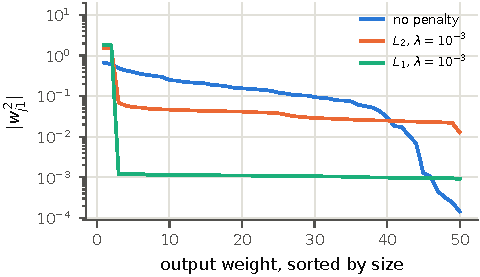
\includegraphics[width=\columnwidth]{runge_sparsity.pdf}
\caption{Both penalties leave two large output weights, and $L_1$ pushes the others further towards zero than $L_2$. Output weights of the 1-50-1 sigmoid network after 3000 epochs of Adam on all 100 observations, sorted by size; median over ten initializations.}\label{fig:sparsity}
\end{figure}
Figure~\ref{fig:sparsity} shows what the two penalties do to the weights of a trained 1-50-1 network. We use $\lambda=10^{-3}$, ten times the value chosen by the one-standard-error rule, because it shows the effect clearly. Without a penalty the output weights spread over three orders of magnitude. Both penalties leave two large weights, so with this much shrinkage two nodes carry the fit. At this strength the $L_2$ fit is clearly degraded, with a training MSE of $36\times10^{-3}$ for one initialization against $14\times10^{-3}$ without penalty, whereas the $L_1$ fit is only slightly worse, at $16\times10^{-3}$. Two nodes is also the size that cross-validation found to be sufficient in Sec.~\ref{sec:res_compare}. The penalties differ in what they do to the rest. $L_2$ shrinks the other 48 weights to a few hundredths, while $L_1$ pushes them all down to about $10^{-3}$. They do not become exactly zero, because a subgradient step moves a weight past zero rather than onto it. This resembles the Lasso, which sets small polynomial coefficients to zero, while Ridge only shrinks them.

\section{Measurements behind the explanations}\label{app:measurements}
Several explanations in Secs.~\ref{sec:results} and \ref{sec:discussion} are tested with the measurements in Table~\ref{tab:measurements}. They use the training and validation data only. Where the networks are those of a figure, they are rerun with the same settings and seeds, and the reruns reproduce the saved curves of that figure exactly.

\section{Use of AI/LLM tools}\label{app:llm}
This declaration follows the course guidelines \cite{LLMGuidelines2026}. For report text the guidelines allow only level 0 (none) and level 1 (language only: spell-check, grammar, minor phrasing); any larger contribution to the writing is not permitted. For code the guidelines define five levels, 0 (none) to 4 (the model wrote most of a file, which the author then adapted, tested and commented).

\subsection{Tools used}
Claude Opus 5.5 (Anthropic), through the Claude Code desktop application, November 2026, for everything listed below. It worked directly in the project folder: it read the course material, wrote and ran code, inspected the results and wrote text. The files reused from the earlier study also contain work by OpenAI Codex (October 2026), as declared in that report \cite{Ozdber2026}.

\subsection{How the work was produced}

I produced this report and its code during the project month, working with Claude as my coding and language tool. I derived the equations of Sec.~\ref{sec:theory} and Appendix~\ref{app:pairs} by hand and checked them against Chapters 4, 5 and 8 of the lecture notes before typing them in. I wrote the core of \texttt{network.py} --- the activations, the costs, the feed-forward pass, the backward pass and the penalties --- reusing the optimizers of our earlier study unchanged, and checked each piece against the tests of Table~\ref{tab:verification} as I wrote it. Claude helped me debug the backward loop, and drafted the parallelisation, input--output, plotting, test and notebook boilerplate. I chose the grids, batches and folds, the one-standard-error rule, the panels of every figure and the models carried to the test sets, and I ran every experiment listed in Sec.~\ref{sec:results}. The text is my own writing: early passages were drafted with Claude as the tool, and I rewrote each section in my own words, checking every number against the files under \texttt{results/}. Claude's final audit of the report is described under Errors below, and the session history is in the repository.

\subsection{Text}
{\small\renewcommand{\arraystretch}{1.15}
\noindent\begin{tabular}{@{}p{0.27\columnwidth}cp{0.6\columnwidth}@{}}
\hline
Section & Level & Notes\\ \hline
Abstract & 1 & Written from my notes on the results; language checked.\\
Introduction & 1 & My own writing; language checked.\\
Theory & 0 & Equations derived by hand first, then typed; written independently.\\
Methods & 1 & My own writing; language checked.\\
Results, captions, tables & 1 & Written from my summaries of the runs; every number read from \texttt{results/}.\\
\end{tabular}\par\nointerlineskip
% The tables of this appendix are split in two so that they can continue in the next column;
% \makebox keeps the middle column as wide as its header "Level" in the first part.
\newlength{\levelwidth}\settowidth{\levelwidth}{Level}
\noindent\begin{tabular}{@{}p{0.27\columnwidth}cp{0.6\columnwidth}@{}}
Discussion & \makebox[\levelwidth]{1} & My own writing; language checked.\\
Conclusions & 1 & Written from my notes on the results; language checked.\\
Appendices A and B & 0 & Derivation and analysis done by hand; the expressions in A are tested numerically against automatic differentiation.\\
This appendix & 1 & Structure follows the guidelines; my own words.\\
References & 1 & The list was compiled with Claude and each entry checked against Crossref or the publisher's page; I read the sources I cite.\\
\hline
\end{tabular}}

\subsection{Code}
Paths are relative to \texttt{Code/}. Every function with LLM assistance carries an \texttt{LLM-assisted} tag in its docstring or in the docstring of its module, stating the role; reused files keep the tags they already had, and a reused file carries the level the earlier study declared for it.


\medskip
{\small\renewcommand{\arraystretch}{1.15}
\noindent\begin{tabular}{@{}p{0.27\columnwidth}cp{0.6\columnwidth}@{}}
\hline
File & Level & Role of the LLM\\ \hline
\texttt{network.py} & 2 & The activations, costs, feed-forward pass, backward pass and penalties are mine; Claude helped debug the backward loop.\\
\texttt{optimizers.py} & 3 & Reused unchanged from the earlier study, which declared it at this level: the update rules, gradients and cost functions are mine; the class structure and driver loops were drafted with Claude there (declared in \cite{Ozdber2026}).\\
\texttt{estimators.py} & 2 & The estimator interface and rules are mine; the endpoints drafted with Claude.\\
\texttt{mnist\_\allowbreak data.py} & 2 & The loading, splitting and scaling rules are mine; the download, cache and checksum helpers drafted with Claude.\\
\texttt{runge\_\allowbreak experiments.py} & 2 & The grids, folds, one-standard-error rule and protocol are mine; the parallelisation and JSON input--output drafted with Claude.\\
\texttt{mnist\_\allowbreak experiments.py} & 2 & The splits, settings and evaluation protocol are mine; the parallelisation and probes drafted with Claude.\\
\texttt{verification\allowbreak.py} & 2 & The checks follow my derivations and the course reference; the autograd and finite-difference scaffolding drafted with Claude.\\
\end{tabular}\par\nointerlineskip
\settowidth{\levelwidth}{Level}
\noindent\begin{tabular}{@{}p{0.27\columnwidth}cp{0.6\columnwidth}@{}}
\texttt{regression.py} & \makebox[\levelwidth]{4} & Reused unchanged from the earlier study, which declared it at this level: generated with Claude there, with \texttt{checked\_lasso\_path} by OpenAI Codex (declared in \cite{Ozdber2026}).\\
\texttt{plot\_style.py} & \makebox[\levelwidth]{4} & Reused unchanged from the earlier study, which declared it at this level: the style module was generated with Claude there. Only \texttt{load\_results} is new in this project, drafted with Claude.\\
\texttt{figures.py} & \makebox[\levelwidth]{2} & Panel choices and what each figure shows are mine; the matplotlib and seaborn boilerplate drafted with Claude.\\
\texttt{tests/} \emph{(Project 1)} & \makebox[\levelwidth]{4} & \texttt{conftest.py}, \texttt{test\_optimizers.py} and \texttt{test\_regression.py} reused unchanged from the earlier study, which declared them at this level.\\
\texttt{tests/} \emph{(new)} & \makebox[\levelwidth]{2} & The four test files new in this project: the expected values come from my derivations and the course reference; the test scaffolding drafted with Claude.\\
Notebooks & \makebox[\levelwidth]{2} & The cells call the modules; layout and the notes above assisted cells drafted with Claude.\\
\hline
\end{tabular}}


\clearpage
\bibliographystyle{apsrev4-2}
\bibliography{References}

\end{document}
